\documentclass{article}
\usepackage[utf8]{inputenc}

\usepackage{tikz}

\begin{document}

    % Comprimento da aresta do cubo
    \newcommand{\comp}{3}

    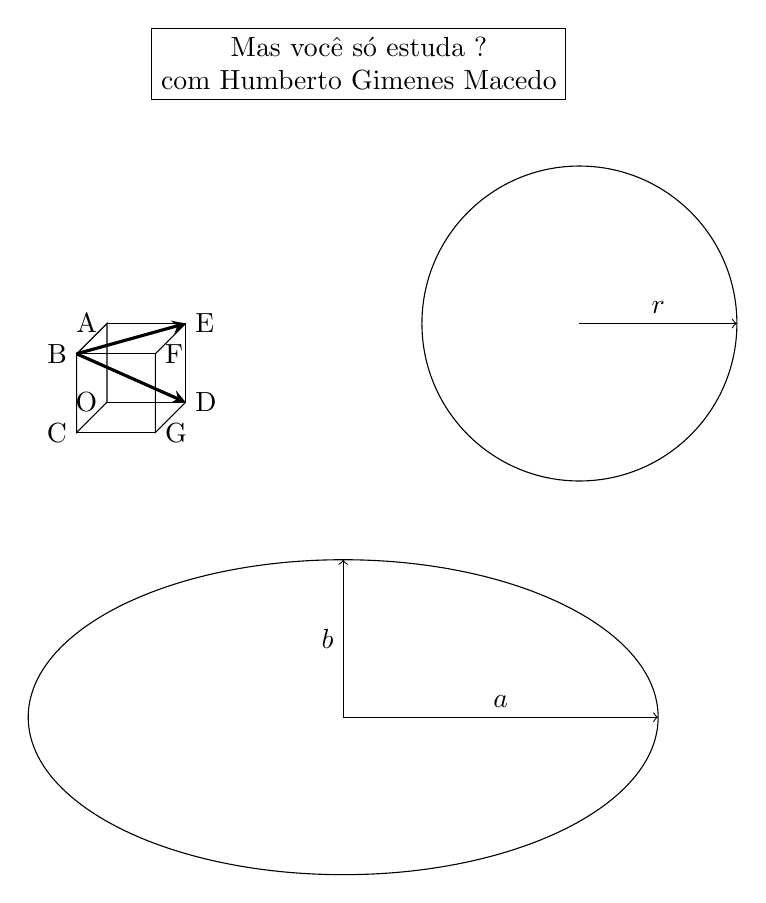
\begin{tikzpicture}
    
        \node[draw, align = center] at (3.2, 4.3) {Mas você só estuda ? \\com Humberto Gimenes Macedo};
        
        % Vértices do cubo e seus rótulos
        \coordinate (O) at (0,0,0);
        \node[left] at (O) {O}; 
        
        \coordinate (A) at (0, \comp, 0);
        \node[left] at (A) {A};
        
        \coordinate (B) at (0, \comp, \comp);
        \node[left] at (B) {B};
        
        \coordinate (C) at (0, 0, \comp);
        \node[left] at (C) {C};
        
        \coordinate (D) at (\comp, 0, 0);
        \node[right] at (D) {D};
        
        \coordinate (E) at (\comp,\comp,0);
        \node[right] at (E) {E};
        
        \coordinate (F) at (\comp,\comp,\comp);
        \node[right] at (F) {F};
        
        \coordinate (G) at (\comp,0,\comp);
        \node[right] at (G) {G};
        
        % Faces do cubo
        \draw (O) -- (A) -- (B) -- (C) -- (O);
        \draw (A) -- (E) -- (D) -- (O);
        \draw (E) -- (F) -- (G) -- (D);
        \draw (F) -- (B);
        \draw (G) -- (C);
        
        % Vetores
        \draw[-stealth, line width = 0.4mm] (B) -- (D);
        \draw[-stealth, line width = 0.4mm] (B) -- (E);
        
        % Circunferência 
        \draw (6, 1) circle (2);
        \draw[->] (6, 1) -- (8, 1) node[midway, above]{$r$};
        
        % Elipse
        \draw (3, -4) ellipse (4 and 2);
        \draw[->] (3, -4) -- (7, -4) node[midway, above]{$a$};
        \draw[->] (3, -4) -- (3, -2) node[midway, left]{$b$};
    \end{tikzpicture}
\end{document}
